% Figure from MATH 556 notes, section 37. Compile with the notes preamble.
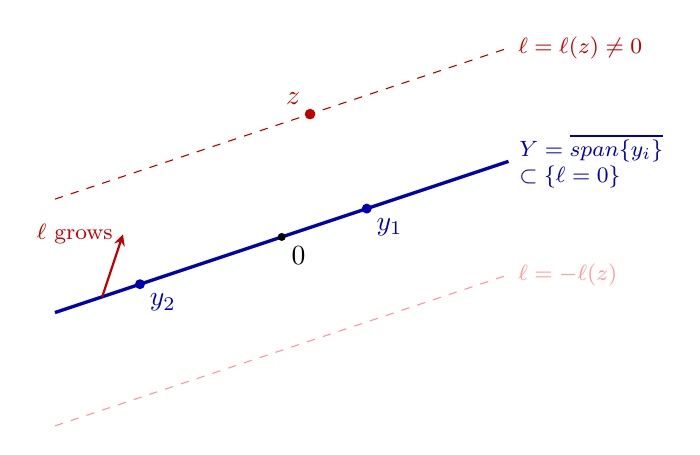
\begin{tikzpicture}[scale=1.2, >=stealth]
    \draw[dashed, red!75!black] (-2.4,0.4) -- (2.4,2.0) node[right, font=\footnotesize] {$\ell = \ell(z) \neq 0$};
    \draw[dashed, red!40] (-2.4,-2.0) -- (2.4,-0.4) node[right, font=\footnotesize] {$\ell = -\ell(z)$};
    \draw[very thick, blue!70!black] (-2.4,-0.8) -- (2.4,0.8) node[right, align=left, font=\footnotesize] {$Y = \overline{\operatorname{span}\{y_i\}}$\\ $\subset \{\ell = 0\}$};
    \fill (0,0) circle (1.2pt) node[below right] {$0$};
    \fill[blue!70!black] (0.9,0.3) circle (1.5pt) node[below right] {$y_1$};
    \fill[blue!70!black] (-1.5,-0.5) circle (1.5pt) node[below right] {$y_2$};
    \fill[red!75!black] (0.3,1.3) circle (1.6pt) node[above left] {$z$};
    \draw[->, thick, red!75!black] (-1.9,-0.633) -- (-1.68,0.027) node[left, font=\footnotesize] {$\ell$ grows};
\end{tikzpicture}
